% Options for packages loaded elsewhere
\PassOptionsToPackage{unicode}{hyperref}
\PassOptionsToPackage{hyphens}{url}
\PassOptionsToPackage{dvipsnames,svgnames,x11names}{xcolor}
%
\documentclass[
  letterpaper,
  DIV=11,
  numbers=noendperiod]{scrreprt}

\usepackage{amsmath,amssymb}
\usepackage{iftex}
\ifPDFTeX
  \usepackage[T1]{fontenc}
  \usepackage[utf8]{inputenc}
  \usepackage{textcomp} % provide euro and other symbols
\else % if luatex or xetex
  \usepackage{unicode-math}
  \defaultfontfeatures{Scale=MatchLowercase}
  \defaultfontfeatures[\rmfamily]{Ligatures=TeX,Scale=1}
\fi
\usepackage{lmodern}
\ifPDFTeX\else  
    % xetex/luatex font selection
\fi
% Use upquote if available, for straight quotes in verbatim environments
\IfFileExists{upquote.sty}{\usepackage{upquote}}{}
\IfFileExists{microtype.sty}{% use microtype if available
  \usepackage[]{microtype}
  \UseMicrotypeSet[protrusion]{basicmath} % disable protrusion for tt fonts
}{}
\makeatletter
\@ifundefined{KOMAClassName}{% if non-KOMA class
  \IfFileExists{parskip.sty}{%
    \usepackage{parskip}
  }{% else
    \setlength{\parindent}{0pt}
    \setlength{\parskip}{6pt plus 2pt minus 1pt}}
}{% if KOMA class
  \KOMAoptions{parskip=half}}
\makeatother
\usepackage{xcolor}
\setlength{\emergencystretch}{3em} % prevent overfull lines
\setcounter{secnumdepth}{5}
% Make \paragraph and \subparagraph free-standing
\makeatletter
\ifx\paragraph\undefined\else
  \let\oldparagraph\paragraph
  \renewcommand{\paragraph}{
    \@ifstar
      \xxxParagraphStar
      \xxxParagraphNoStar
  }
  \newcommand{\xxxParagraphStar}[1]{\oldparagraph*{#1}\mbox{}}
  \newcommand{\xxxParagraphNoStar}[1]{\oldparagraph{#1}\mbox{}}
\fi
\ifx\subparagraph\undefined\else
  \let\oldsubparagraph\subparagraph
  \renewcommand{\subparagraph}{
    \@ifstar
      \xxxSubParagraphStar
      \xxxSubParagraphNoStar
  }
  \newcommand{\xxxSubParagraphStar}[1]{\oldsubparagraph*{#1}\mbox{}}
  \newcommand{\xxxSubParagraphNoStar}[1]{\oldsubparagraph{#1}\mbox{}}
\fi
\makeatother

\usepackage{color}
\usepackage{fancyvrb}
\newcommand{\VerbBar}{|}
\newcommand{\VERB}{\Verb[commandchars=\\\{\}]}
\DefineVerbatimEnvironment{Highlighting}{Verbatim}{commandchars=\\\{\}}
% Add ',fontsize=\small' for more characters per line
\usepackage{framed}
\definecolor{shadecolor}{RGB}{241,243,245}
\newenvironment{Shaded}{\begin{snugshade}}{\end{snugshade}}
\newcommand{\AlertTok}[1]{\textcolor[rgb]{0.68,0.00,0.00}{#1}}
\newcommand{\AnnotationTok}[1]{\textcolor[rgb]{0.37,0.37,0.37}{#1}}
\newcommand{\AttributeTok}[1]{\textcolor[rgb]{0.40,0.45,0.13}{#1}}
\newcommand{\BaseNTok}[1]{\textcolor[rgb]{0.68,0.00,0.00}{#1}}
\newcommand{\BuiltInTok}[1]{\textcolor[rgb]{0.00,0.23,0.31}{#1}}
\newcommand{\CharTok}[1]{\textcolor[rgb]{0.13,0.47,0.30}{#1}}
\newcommand{\CommentTok}[1]{\textcolor[rgb]{0.37,0.37,0.37}{#1}}
\newcommand{\CommentVarTok}[1]{\textcolor[rgb]{0.37,0.37,0.37}{\textit{#1}}}
\newcommand{\ConstantTok}[1]{\textcolor[rgb]{0.56,0.35,0.01}{#1}}
\newcommand{\ControlFlowTok}[1]{\textcolor[rgb]{0.00,0.23,0.31}{\textbf{#1}}}
\newcommand{\DataTypeTok}[1]{\textcolor[rgb]{0.68,0.00,0.00}{#1}}
\newcommand{\DecValTok}[1]{\textcolor[rgb]{0.68,0.00,0.00}{#1}}
\newcommand{\DocumentationTok}[1]{\textcolor[rgb]{0.37,0.37,0.37}{\textit{#1}}}
\newcommand{\ErrorTok}[1]{\textcolor[rgb]{0.68,0.00,0.00}{#1}}
\newcommand{\ExtensionTok}[1]{\textcolor[rgb]{0.00,0.23,0.31}{#1}}
\newcommand{\FloatTok}[1]{\textcolor[rgb]{0.68,0.00,0.00}{#1}}
\newcommand{\FunctionTok}[1]{\textcolor[rgb]{0.28,0.35,0.67}{#1}}
\newcommand{\ImportTok}[1]{\textcolor[rgb]{0.00,0.46,0.62}{#1}}
\newcommand{\InformationTok}[1]{\textcolor[rgb]{0.37,0.37,0.37}{#1}}
\newcommand{\KeywordTok}[1]{\textcolor[rgb]{0.00,0.23,0.31}{\textbf{#1}}}
\newcommand{\NormalTok}[1]{\textcolor[rgb]{0.00,0.23,0.31}{#1}}
\newcommand{\OperatorTok}[1]{\textcolor[rgb]{0.37,0.37,0.37}{#1}}
\newcommand{\OtherTok}[1]{\textcolor[rgb]{0.00,0.23,0.31}{#1}}
\newcommand{\PreprocessorTok}[1]{\textcolor[rgb]{0.68,0.00,0.00}{#1}}
\newcommand{\RegionMarkerTok}[1]{\textcolor[rgb]{0.00,0.23,0.31}{#1}}
\newcommand{\SpecialCharTok}[1]{\textcolor[rgb]{0.37,0.37,0.37}{#1}}
\newcommand{\SpecialStringTok}[1]{\textcolor[rgb]{0.13,0.47,0.30}{#1}}
\newcommand{\StringTok}[1]{\textcolor[rgb]{0.13,0.47,0.30}{#1}}
\newcommand{\VariableTok}[1]{\textcolor[rgb]{0.07,0.07,0.07}{#1}}
\newcommand{\VerbatimStringTok}[1]{\textcolor[rgb]{0.13,0.47,0.30}{#1}}
\newcommand{\WarningTok}[1]{\textcolor[rgb]{0.37,0.37,0.37}{\textit{#1}}}

\providecommand{\tightlist}{%
  \setlength{\itemsep}{0pt}\setlength{\parskip}{0pt}}\usepackage{longtable,booktabs,array}
\usepackage{calc} % for calculating minipage widths
% Correct order of tables after \paragraph or \subparagraph
\usepackage{etoolbox}
\makeatletter
\patchcmd\longtable{\par}{\if@noskipsec\mbox{}\fi\par}{}{}
\makeatother
% Allow footnotes in longtable head/foot
\IfFileExists{footnotehyper.sty}{\usepackage{footnotehyper}}{\usepackage{footnote}}
\makesavenoteenv{longtable}
\usepackage{graphicx}
\makeatletter
\def\maxwidth{\ifdim\Gin@nat@width>\linewidth\linewidth\else\Gin@nat@width\fi}
\def\maxheight{\ifdim\Gin@nat@height>\textheight\textheight\else\Gin@nat@height\fi}
\makeatother
% Scale images if necessary, so that they will not overflow the page
% margins by default, and it is still possible to overwrite the defaults
% using explicit options in \includegraphics[width, height, ...]{}
\setkeys{Gin}{width=\maxwidth,height=\maxheight,keepaspectratio}
% Set default figure placement to htbp
\makeatletter
\def\fps@figure{htbp}
\makeatother
% definitions for citeproc citations
\NewDocumentCommand\citeproctext{}{}
\NewDocumentCommand\citeproc{mm}{%
  \begingroup\def\citeproctext{#2}\cite{#1}\endgroup}
\makeatletter
 % allow citations to break across lines
 \let\@cite@ofmt\@firstofone
 % avoid brackets around text for \cite:
 \def\@biblabel#1{}
 \def\@cite#1#2{{#1\if@tempswa , #2\fi}}
\makeatother
\newlength{\cslhangindent}
\setlength{\cslhangindent}{1.5em}
\newlength{\csllabelwidth}
\setlength{\csllabelwidth}{3em}
\newenvironment{CSLReferences}[2] % #1 hanging-indent, #2 entry-spacing
 {\begin{list}{}{%
  \setlength{\itemindent}{0pt}
  \setlength{\leftmargin}{0pt}
  \setlength{\parsep}{0pt}
  % turn on hanging indent if param 1 is 1
  \ifodd #1
   \setlength{\leftmargin}{\cslhangindent}
   \setlength{\itemindent}{-1\cslhangindent}
  \fi
  % set entry spacing
  \setlength{\itemsep}{#2\baselineskip}}}
 {\end{list}}
\usepackage{calc}
\newcommand{\CSLBlock}[1]{\hfill\break\parbox[t]{\linewidth}{\strut\ignorespaces#1\strut}}
\newcommand{\CSLLeftMargin}[1]{\parbox[t]{\csllabelwidth}{\strut#1\strut}}
\newcommand{\CSLRightInline}[1]{\parbox[t]{\linewidth - \csllabelwidth}{\strut#1\strut}}
\newcommand{\CSLIndent}[1]{\hspace{\cslhangindent}#1}

\usepackage{booktabs}
\usepackage{longtable}
\usepackage{array}
\usepackage{multirow}
\usepackage{wrapfig}
\usepackage{float}
\usepackage{colortbl}
\usepackage{pdflscape}
\usepackage{tabu}
\usepackage{threeparttable}
\usepackage{threeparttablex}
\usepackage[normalem]{ulem}
\usepackage{makecell}
\usepackage{xcolor}
\KOMAoption{captions}{tableheading}
\makeatletter
\@ifpackageloaded{tcolorbox}{}{\usepackage[skins,breakable]{tcolorbox}}
\@ifpackageloaded{fontawesome5}{}{\usepackage{fontawesome5}}
\definecolor{quarto-callout-color}{HTML}{909090}
\definecolor{quarto-callout-note-color}{HTML}{0758E5}
\definecolor{quarto-callout-important-color}{HTML}{CC1914}
\definecolor{quarto-callout-warning-color}{HTML}{EB9113}
\definecolor{quarto-callout-tip-color}{HTML}{00A047}
\definecolor{quarto-callout-caution-color}{HTML}{FC5300}
\definecolor{quarto-callout-color-frame}{HTML}{acacac}
\definecolor{quarto-callout-note-color-frame}{HTML}{4582ec}
\definecolor{quarto-callout-important-color-frame}{HTML}{d9534f}
\definecolor{quarto-callout-warning-color-frame}{HTML}{f0ad4e}
\definecolor{quarto-callout-tip-color-frame}{HTML}{02b875}
\definecolor{quarto-callout-caution-color-frame}{HTML}{fd7e14}
\makeatother
\makeatletter
\@ifpackageloaded{bookmark}{}{\usepackage{bookmark}}
\makeatother
\makeatletter
\@ifpackageloaded{caption}{}{\usepackage{caption}}
\AtBeginDocument{%
\ifdefined\contentsname
  \renewcommand*\contentsname{Table of contents}
\else
  \newcommand\contentsname{Table of contents}
\fi
\ifdefined\listfigurename
  \renewcommand*\listfigurename{List of Figures}
\else
  \newcommand\listfigurename{List of Figures}
\fi
\ifdefined\listtablename
  \renewcommand*\listtablename{List of Tables}
\else
  \newcommand\listtablename{List of Tables}
\fi
\ifdefined\figurename
  \renewcommand*\figurename{Figure}
\else
  \newcommand\figurename{Figure}
\fi
\ifdefined\tablename
  \renewcommand*\tablename{Table}
\else
  \newcommand\tablename{Table}
\fi
}
\@ifpackageloaded{float}{}{\usepackage{float}}
\floatstyle{ruled}
\@ifundefined{c@chapter}{\newfloat{codelisting}{h}{lop}}{\newfloat{codelisting}{h}{lop}[chapter]}
\floatname{codelisting}{Listing}
\newcommand*\listoflistings{\listof{codelisting}{List of Listings}}
\makeatother
\makeatletter
\makeatother
\makeatletter
\@ifpackageloaded{caption}{}{\usepackage{caption}}
\@ifpackageloaded{subcaption}{}{\usepackage{subcaption}}
\makeatother

\ifLuaTeX
  \usepackage{selnolig}  % disable illegal ligatures
\fi
\usepackage{bookmark}

\IfFileExists{xurl.sty}{\usepackage{xurl}}{} % add URL line breaks if available
\urlstyle{same} % disable monospaced font for URLs
\hypersetup{
  pdftitle={Statistics-II (B.Sc.)},
  pdfauthor={Prof.~Dr.~Dominik Liebl},
  colorlinks=true,
  linkcolor={blue},
  filecolor={Maroon},
  citecolor={Blue},
  urlcolor={Blue},
  pdfcreator={LaTeX via pandoc}}


\title{Statistics-II (B.Sc.)}
\author{Prof.~Dr.~Dominik Liebl}
\date{Last Updated on October 21, 2025}

\begin{document}
\maketitle

\renewcommand*\contentsname{Table of contents}
{
\hypersetup{linkcolor=}
\setcounter{tocdepth}{2}
\tableofcontents
}

\bookmarksetup{startatroot}

\chapter*{Organization of the Course}\label{organization-of-the-course}
\addcontentsline{toc}{chapter}{Organization of the Course}

\markboth{Organization of the Course}{Organization of the Course}

\subsection*{Timetable}\label{timetable}
\addcontentsline{toc}{subsection}{Timetable}

\begin{table}
\centering
\begin{tabular}[t]{l|l|l}
\hline
Day & Time & Lecture Hall\\
\hline
Monday & 14:15-15:45 & Lecture Hall K\\
\hline
Thursday & 15:45-16:15 & Lecture Hall K\\
\hline
\end{tabular}
\end{table}

\subsection*{Link to this Lecture}\label{link-to-this-lecture}
\addcontentsline{toc}{subsection}{Link to this Lecture}

\begin{center}

\includegraphics[width=0.25\textwidth,height=\textheight]{images/lecture_page_linke.png}
\end{center}

\url{https://www.dliebl.com/Script-Statistics-2/}

\subsection*{Lecture Material}\label{lecture-material}
\addcontentsline{toc}{subsection}{Lecture Material}

\begin{itemize}
\tightlist
\item
  This online script
\item
  \href{https://www.dropbox.com/scl/fo/omfqxytalaiyx4kd0kv4o/AE7EhUu8W3dJPvaA_ETDlQM?rlkey=w6v0am29ypq38gt4xpzy230bj&st=8p60234i&dl=0}{Folder
  containing \texttt{R}-Scripts}
\item
  \href{https://www.dropbox.com/scl/fi/vnzws3xkbs2ojd5mfcdxr/CASA_eWhiteboard_2526_annotated.pdf?rlkey=ny3rnruqrsyyy1j4i2z3rdoek&st=djjulif7&dl=0}{eWhiteboard}
\end{itemize}

\subsection*{Literature}\label{literature}
\addcontentsline{toc}{subsection}{Literature}

\begin{itemize}
\tightlist
\item
  \href{https://link.springer.com/book/10.1007/978-3-662-67526-7}{Statistik:
  Der Weg zur Datenanalyse}
\item
  \href{https://press.princeton.edu/books/hardcover/9780691235943/probability-and-statistics-for-economists?srsltid=AfmBOopn6HIW0Y1Edtu1W8VdiDmPN6PfNiCwHmyTBjQEHqM5i3W4ysVK}{Probability
  and Statistics for Economists}
\end{itemize}

%% Colorbox within equation-environments:
\newcommand{\highlight}[2][yellow]{\mathchoice%
  {\colorbox{#1}{$\displaystyle#2$}}%
  {\colorbox{#1}{$\displaystyle#2$}}%
  {\colorbox{#1}{$\displaystyle#2$}}%
  }%

\bookmarksetup{startatroot}

\chapter{\texorpdfstring{\(\mathrm{p}\)-Values: Challenges for
Hypothesis
Testing}{\textbackslash mathrm\{p\}-Values: Challenges for Hypothesis Testing}}\label{mathrmp-values-challenges-for-hypothesis-testing}

\subsubsection*{\texorpdfstring{🎯 \textbf{Lecture
Goals}}{🎯 Lecture Goals}}\label{lecture-goals}
\addcontentsline{toc}{subsubsection}{🎯 \textbf{Lecture Goals}}

\begin{itemize}
\item
  \textbf{How} do \(\mathrm{p}\)-values work?

  \begin{itemize}
  \tightlist
  \item
    Today: {two-sided \(t\)-test}
  \end{itemize}
\item
  \textbf{Why} are \(\mathrm{p}\)-values a challenge for hypothesis
  testing?
\item
  \textbf{What} alternatives are there?
\end{itemize}

\section{Real-Example: Marketing
Campaign}\label{real-example-marketing-campaign}

Marketing campaign in \(n=5\) stores (paired sample):

\begin{longtable}[]{@{}llll@{}}
\toprule\noalign{}
Store & Sales Before & Sales After & Difference (After \(-\) Before) \\
\midrule\noalign{}
\endhead
\bottomrule\noalign{}
\endlastfoot
\(1\) & \(4.86\) & \(5.50\) & \(X_{1,obs}=0.64\) \\
\(2\) & \(4.96\) & \(4.24\) & \(X_{2,obs}=-0.72\) \\
\(3\) & \(6.01\) & \(5.78\) & \(X_{3,obs}=-0.23\) \\
\(4\) & \(4.84\) & \(5.75\) & \(X_{4,obs}=0.91\) \\
\(5\) & \(2.84\) & \(3.90\) & \(X_{5,obs}=1.06\) \\
\end{longtable}

Figure~\ref{fig-diffData} shows the observed sales differences \[
\{X_{1,obs},X_{2,obs},X_{3,obs},X_{4,obs},X_{5,obs}\}.
\]

\begin{figure}

\centering{

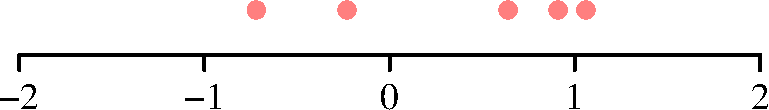
\includegraphics{Ch_pValues_files/figure-pdf/fig-diffData-1.pdf}

}

\caption{\label{fig-diffData}Sales differences (sales after minus before
the marketing campaign).}

\end{figure}%

\begin{itemize}
\item
  \textbf{Research Question:} Was the marketing campaign successful? Did
  it show a tendency (location-shift) toward \emph{significantly} higher
  or lower sales?
\item
  \textbf{Statistical Reformulation:} Is the mean of \(X_1,\dots,X_n\)
  different from zero?
\item
  \textbf{Testing problem:} \(\hspace{1cm}H_0\colon \mu = 0\quad\)
  versus \(\quad H_1\colon \mu \neq 0\)
\end{itemize}

\begin{tcolorbox}[enhanced jigsaw, opacityback=0, colback=white, colframe=quarto-callout-note-color-frame, breakable, rightrule=.15mm, arc=.35mm, left=2mm, bottomrule=.15mm, toprule=.15mm, leftrule=.75mm]

\textbf{Assumption:} There are no systematic differences (mean-shifts)
between sales before and after the marketing campaign, other than the
potential impact of the campaign itself.

\end{tcolorbox}

\section{\texorpdfstring{Short Repetition: Two-Sided
\(t\)-Test}{Short Repetition: Two-Sided t-Test}}\label{short-repetition-two-sided-t-test}

\begin{tcolorbox}[enhanced jigsaw, opacityback=0, colback=white, colframe=quarto-callout-note-color-frame, breakable, rightrule=.15mm, arc=.35mm, left=2mm, bottomrule=.15mm, toprule=.15mm, leftrule=.75mm]

\textbf{More Details:} See our lecture on hypothesis testing for more
details.

\end{tcolorbox}

Statistical hypothesis:

\(\displaystyle H_0\colon \mu = 0\quad\) versus
\(\displaystyle \quad H_1\colon \mu \neq 0\)

\(t\)-test statistic: \[
\mathrm{T} = \frac{\sqrt{n}(\bar{X} - 0)}{s}\overset{H_0}{\sim} t_{n-1},
\] where \begin{align*}
\bar{X}&=\frac{1}{n}\sum_{i=1}^n X_i\\
s      &= \sqrt{\frac{1}{n-1}\sum_{i=1}^n(X_i-\bar{X})}
\end{align*}

denote the empirical mean and the empirical standard deviation.

\begin{tcolorbox}[enhanced jigsaw, opacityback=0, colback=white, colframe=quarto-callout-note-color-frame, breakable, rightrule=.15mm, arc=.35mm, left=2mm, bottomrule=.15mm, toprule=.15mm, leftrule=.75mm]

\textbf{Assumptions:}

\begin{itemize}
\item
  Random (iid) sample:
  \(X_1,\dots,X_n\overset{\operatorname{iid}}{\sim}X\)
\item
  For small sample sizes: \(X\sim\mathcal{N}(\mu, \sigma^2)\)
\item
  For large sample sizes (CLT, \(n\to\infty\)): \[
  \mathrm{E}(X)=\mu\quad\text{and}\quad \mathrm{Var}(X)=\sigma^2
  \]
\end{itemize}

\end{tcolorbox}

\textbf{Observed (\emph{obs}) realization (marketing campaign):}

\[
\mathrm{T}_{\mathrm{obs}} = \frac{\sqrt{n}(\bar{X}_{\mathrm{obs}} - 0)}{s_{\mathrm{obs}}} = 0.84
\]

\begin{itemize}
\tightlist
\item
  \(\bar{X}_{\mathrm{obs}}=\frac{1}{5}\sum_{i=1}^5 X_{i,obs} = 0.30\)
\item
  \(s_{\mathrm{obs}} = \sqrt{\frac{1}{5-1}\sum_{i=1}^5(X_{i,obs}-\bar{X}_{\mathrm{obs}})} = 0.80\)
\end{itemize}

\subsubsection*{\texorpdfstring{\textbf{Critical Values
\(\phantom{\mathrm{p}}\)}}{Critical Values \textbackslash phantom\{\textbackslash mathrm\{p\}\}}}\label{critical-values-phantommathrmp}
\addcontentsline{toc}{subsubsection}{\textbf{Critical Values
\(\phantom{\mathrm{p}}\)}}

\begin{tcolorbox}[enhanced jigsaw, opacityback=0, colback=white, colframe=quarto-callout-note-color-frame, breakable, rightrule=.15mm, arc=.35mm, left=2mm, bottomrule=.15mm, toprule=.15mm, leftrule=.75mm]

\textbf{Critical Values:} The critical values --- the \((1-\alpha/2)\)-
and the \(\alpha/2\)-quantiles of the \(t\)-distribution with
\(\operatorname{df}=n-1\) --- define the rejection regions for a given
significance level \(0<\alpha<1\).

\end{tcolorbox}

Marketing campaign data:

Density function of the \(t_{\operatorname{df}}\) distribution with
\(\operatorname{df}=4\)

\begin{center}
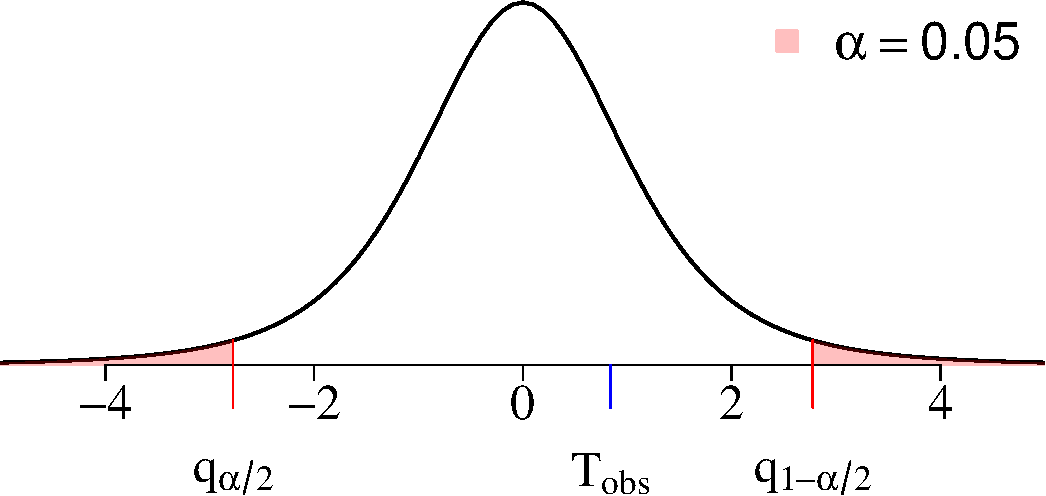
\includegraphics[width=7in,height=\textheight]{Ch_pValues_files/figure-pdf/unnamed-chunk-3-1.pdf}
\end{center}

\section{\texorpdfstring{Two-Sided
\(\mathrm{p}\)-Value}{Two-Sided \textbackslash mathrm\{p\}-Value}}\label{two-sided-mathrmp-value}

\begin{tcolorbox}[enhanced jigsaw, opacityback=0, colback=white, colframe=quarto-callout-note-color-frame, breakable, rightrule=.15mm, arc=.35mm, left=2mm, bottomrule=.15mm, toprule=.15mm, leftrule=.75mm]

\textbf{\(\mathrm{p}\)-Value:} The \(\mathrm{p}\)-value is the
probability of observing a test statistic \(\mathrm{T}\) as extreme as
\(\mathrm{T}_{\mathrm{obs}}\) or more extreme (in the direction(s) of
the alternative hypothesis) than \(\mathrm{T}_{\mathrm{obs}}\), given
the null hypothesis (\(H_0\)) is true.

\begin{itemize}
\tightlist
\item
  \textbf{Two-Sided \(\mathrm{p}\)-Value:}
  \[\displaystyle\mathrm{p}_{\mathrm{obs}} = \mathrm{P}\big(\,|\mathrm{T}|\,\geq |\mathrm{T}_{\mathrm{obs}}|\;\big|\;H_0\;\text{is true}\big)\]
\end{itemize}

\end{tcolorbox}

Marketing campaign data:

Density function of the \(t_{\operatorname{df}}\) distribution with
\(\operatorname{df}=4\)

\begin{center}
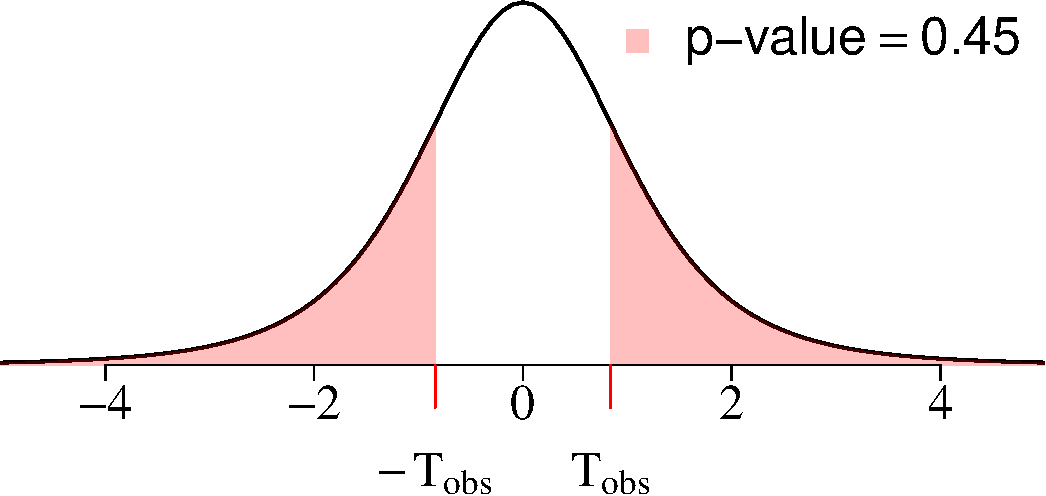
\includegraphics[width=7in,height=\textheight]{Ch_pValues_files/figure-pdf/unnamed-chunk-4-1.pdf}
\end{center}

\section{\texorpdfstring{Two-Sided
\(\mathrm{p}\)-Value}{Two-Sided \textbackslash mathrm\{p\}-Value}}\label{two-sided-mathrmp-value-1}

\begin{tcolorbox}[enhanced jigsaw, opacityback=0, colback=white, colframe=quarto-callout-note-color-frame, breakable, rightrule=.15mm, arc=.35mm, left=2mm, bottomrule=.15mm, toprule=.15mm, leftrule=.75mm]

\textbf{\(\mathrm{p}\)-Value:} The \(\mathrm{p}\)-value is the
probability of observing a test statistic \(\mathrm{T}\) as extreme as
\(\mathrm{T}_{\mathrm{obs}}\) or more extreme (in the direction(s) of
the alternative hypothesis) than \(\mathrm{T}_{\mathrm{obs}}\), given
the null hypothesis (\(H_0\)) is true.

\begin{itemize}
\tightlist
\item
  \textbf{Two-Sided \(\mathrm{p}\)-Value:}
\end{itemize}

\[
\mathrm{p}_{\mathrm{obs}} = \mathrm{P}\big(\highlight{|\mathrm{T}|} \geq |\mathrm{T}_{\mathrm{obs}}|\;\big|\;H_0\;\text{is true}\big)
\]

\end{tcolorbox}

Marketing campaign data:

Density function of the {Half-\(t_{\operatorname{df}}\)} distribution
with \(\operatorname{df}=4\)

\begin{center}
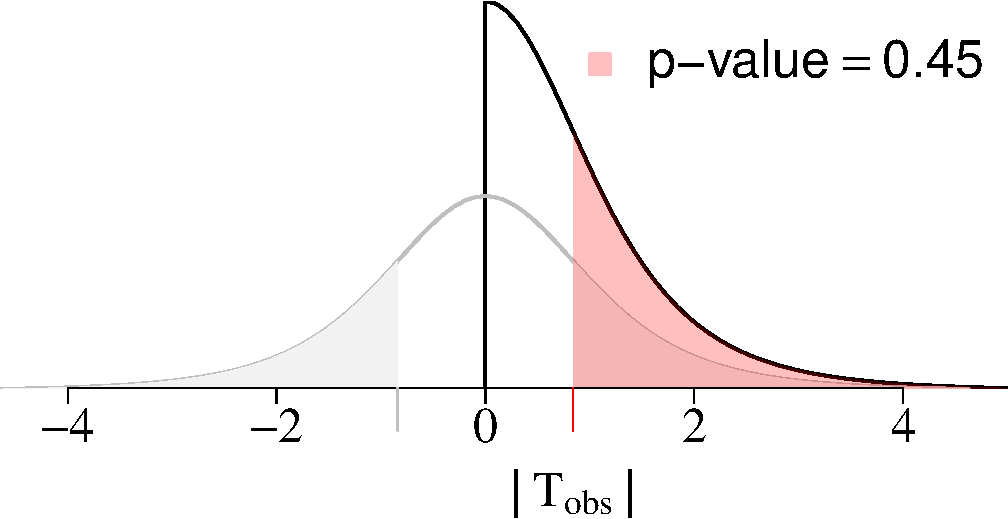
\includegraphics[width=7in,height=\textheight]{Ch_pValues_files/figure-pdf/unnamed-chunk-5-1.pdf}
\end{center}

\section{\texorpdfstring{Two-Sided
\(\mathrm{p}\)-Value}{Two-Sided \textbackslash mathrm\{p\}-Value}}\label{two-sided-mathrmp-value-2}

\textbf{Two-sided \(t\)-test:} \begin{align*}
\mathrm{p}_{\mathrm{obs}} 
& = \mathrm{P}\big(\,|\mathrm{T}|\,\geq |\mathrm{T}_{\mathrm{obs}}|\;\big|\;H_0\;\text{is true}\big)\\[1ex]
& = 1 - \mathrm{P}\big(\highlight{|\mathrm{T}|}\leq |\mathrm{T}_{\mathrm{obs}}|\;\big|\highlight{H_0\;\text{is true}}\big)\\[1ex]
& = 1 - \highlight{\mathrm{F}_{\,\text{Half-}t,n-1}}\big(|\mathrm{T}_{\mathrm{obs}}|\big),
\end{align*} where \(\mathrm{F}_{\,\text{Half-}t,n-1}\) denotes the cdf
of the Half-\(t\) distribution with \(\operatorname{df}=n-1\)

\begin{verbatim}
Warning in mtext(side = 1, text = bquote("|" ~ T[obs] ~ "|"), at =
c(abs(T_obs)), : "hadj" is not a graphical parameter
\end{verbatim}

\begin{center}
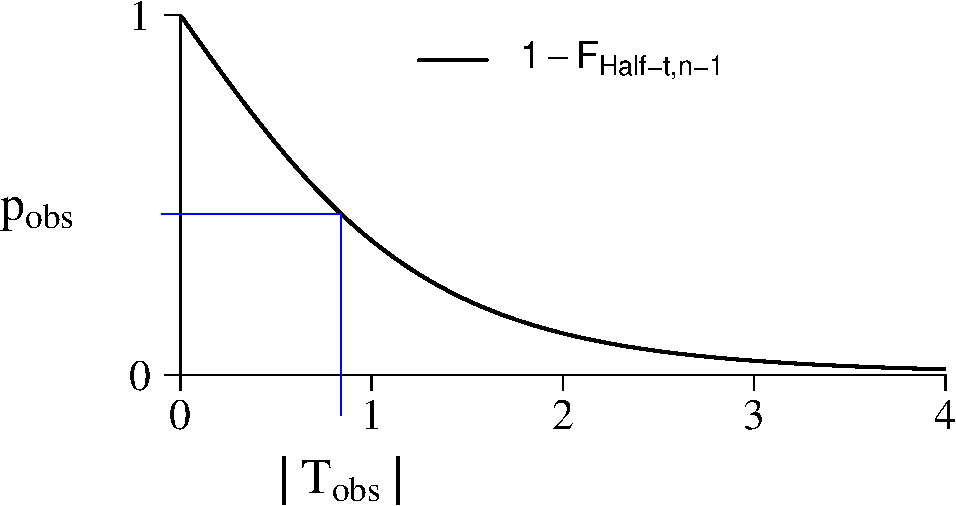
\includegraphics[width=7in,height=\textheight]{Ch_pValues_files/figure-pdf/unnamed-chunk-6-1.pdf}
\end{center}

\begin{Shaded}
\begin{Highlighting}[]
\FunctionTok{library}\NormalTok{(}\StringTok{"extraDistr"}\NormalTok{)}
\NormalTok{df }\OtherTok{\textless{}{-}} \DecValTok{5{-}1}

\DocumentationTok{\#\# 1 minus the distribution function of the Half{-}t}
\NormalTok{p\_obs }\OtherTok{\textless{}{-}} \DecValTok{1} \SpecialCharTok{{-}} \FunctionTok{pht}\NormalTok{(}\AttributeTok{q =} \FunctionTok{abs}\NormalTok{(T\_obs), }\AttributeTok{nu =}\NormalTok{ df)}
\end{Highlighting}
\end{Shaded}

\begin{itemize}
\tightlist
\item
  There's a one-to-one mapping between \(|\mathrm{T}_{obs}|\) and
  \(p_{\mathrm{obs}}\).
\item
  \(p_{\mathrm{obs}}\) effectively measures how extrem the value of
  \(|\mathrm{T}_{obs}|\) is, given that \(H_0\) is true.
\end{itemize}

\section{\texorpdfstring{Two-Sided
\(\mathrm{p}\)-Value}{Two-Sided \textbackslash mathrm\{p\}-Value}}\label{two-sided-mathrmp-value-3}

Marketing campaign data:

\begin{itemize}
\tightlist
\item
  \(|\mathrm{T}_\mathrm{obs}|=0.84\)
\item
  \(\alpha = 0.05\)
\item
  \((1-\alpha/2)\)-quantile of \(t_{4}\colon\)
  \(\mathrm{q}_{1-\alpha/2}=2.78\)
\end{itemize}

\begin{verbatim}
Warning in mtext(side = 1, text = bquote("|" ~ T[obs] ~ "|"), at =
c(abs(T_obs)), : "hadj" is not a graphical parameter
\end{verbatim}

\begin{verbatim}
Warning in mtext(side = 1, text = bquote(q[1 - alpha/2]), at = qt(1 - alpha/2,
: "hadj" is not a graphical parameter
\end{verbatim}

\begin{center}
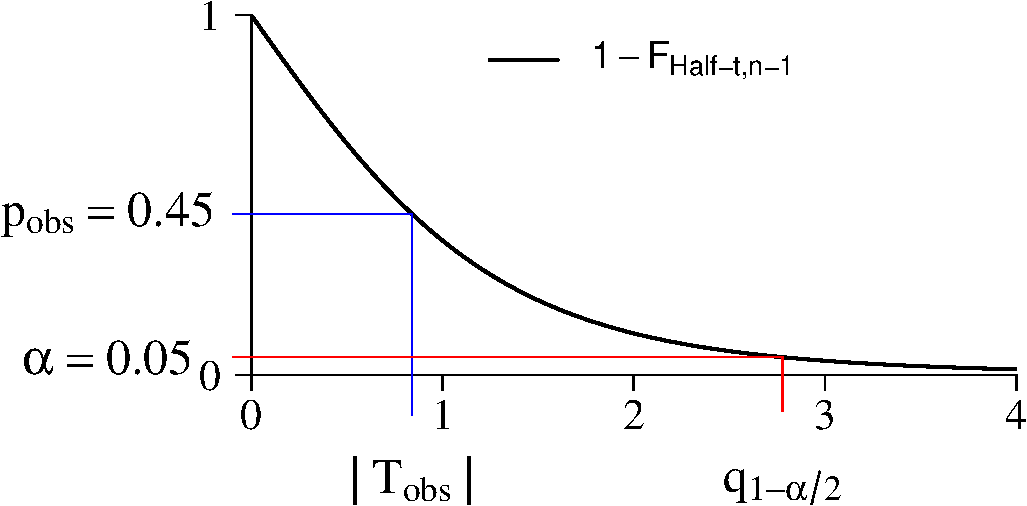
\includegraphics[width=7in,height=\textheight]{Ch_pValues_files/figure-pdf/unnamed-chunk-8-1.pdf}
\end{center}

We fail to reject \(H_0\colon\mu = 0\). That is, we have no statistical
evidence that the marketing campaign showed a tendency toward
\emph{significantly} higher or lower sales.

\begin{tcolorbox}[enhanced jigsaw, opacityback=0, colback=white, colframe=quarto-callout-caution-color-frame, breakable, rightrule=.15mm, arc=.35mm, left=2mm, bottomrule=.15mm, toprule=.15mm, leftrule=.75mm]

⚠️ Failing to reject \(H_0\) does not mean that \(H_0\) is true. It only
means that we do not have enough evidence to reject it.

\end{tcolorbox}

\section{\texorpdfstring{Two-Sided
\(\mathrm{p}\)-Value}{Two-Sided \textbackslash mathrm\{p\}-Value}}\label{two-sided-mathrmp-value-4}

{Equivalent test decisions} at the significance level \(0<\alpha<1\):

\begin{itemize}
\tightlist
\item
  \textbf{Critical values:} Reject \(H_0\colon \mu =0\) if
  {\(\displaystyle|\mathrm{T}_{\mathrm{obs}}| > q_{1-\alpha/2}\)}, where
  \(q_{1-\alpha/2}\) denotes the \((1-\alpha/2)\)-quantile of the
  \(t_{\operatorname{df}}\) distribution.
\end{itemize}

\begin{itemize}
\tightlist
\item
  \textbf{\(\mathrm{p}\)-Values:} Reject \(H_0\colon \mu =0\) if
  {\(\displaystyle\mathrm{p}_{\mathrm{obs}} < \alpha\)}
\end{itemize}

\begin{verbatim}
Warning in mtext(side = 1, text = bquote("|" ~ T[obs] ~ "|"), at =
c(abs(T_2obs)), : "hadj" is not a graphical parameter
\end{verbatim}

\begin{verbatim}
Warning in mtext(side = 1, text = bquote(q[1 - alpha/2]), at = qt(1 - alpha/2,
: "hadj" is not a graphical parameter
\end{verbatim}

\begin{center}
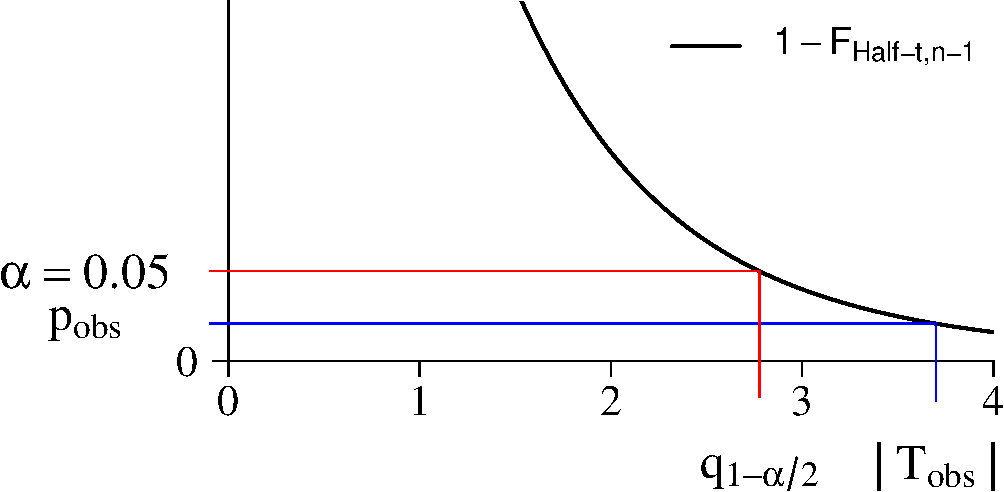
\includegraphics[width=7in,height=\textheight]{Ch_pValues_files/figure-pdf/unnamed-chunk-10-1.pdf}
\end{center}

\section{\texorpdfstring{\(\mathrm{p}\)-Values: Challenges for
Hypothesis
Testing}{\textbackslash mathrm\{p\}-Values: Challenges for Hypothesis Testing}}\label{mathrmp-values-challenges-for-hypothesis-testing-1}

\begin{itemize}
\item
  While the \(\mathrm{p}\)-value can be a useful statistical measure, it
  is commonly misused and misinterpreted. (Wasserstein and Lazar (2016),
  Wasserstein, Schirm, and Lazar (2019))
\item
  ``Scientific method: Statistical errors.'' Nuzzo (2014)
\item
  ScienceNews (Siegfried 2010): ``It's science's dirtiest secret: The
  `scien- tific method' of testing hypotheses by statistical analysis
  stands on a flimsy foundation.''
\end{itemize}

\section{References}\label{references}

\phantomsection\label{refs}
\begin{CSLReferences}{1}{0}
\bibitem[\citeproctext]{ref-nuzzo2014scientific}
Nuzzo, Regina. 2014. {``Scientific Method: {S}tatistical Errors.''}
\emph{Nature} 506 (7487).

\bibitem[\citeproctext]{ref-Wasserstein2016asa}
Wasserstein, Ronald L, and Nicole A Lazar. 2016. {``The ASA Statement on
p-Values: {C}ontext, Process, and Purpose.''} \emph{The American
Statistician}. Taylor \& Francis.

\bibitem[\citeproctext]{ref-wasserstein2019asa}
Wasserstein, Ronald L, Allen L Schirm, and Nicole A Lazar. 2019.
{``Moving to a World Beyond "p\textless{} 0.05".''} \emph{The American
Statistician}. Taylor \& Francis.

\end{CSLReferences}

\section{💡 Tips for Success}\label{tips-for-success}

\begin{itemize}
\tightlist
\item
  Don't just memorize formulas --- focus on understanding \emph{why}
  they work.
\item
  Discuss and collaborate
\end{itemize}




\end{document}
